\documentclass{ximera}  
\title{Newton's Method}  
\begin{document}  
\begin{abstract}  
We give an introduction to finding roots using Newton's Method.
\end{abstract}  
\maketitle

\section{Linear Approximations}

In a calculus course, it is shown that the best linear approximation to a differentiable function $f(x)$ near $x=a$ is given by $L_a(x)=f'(a)(x-a)+f(a)$. We will make use of this general idea to try to approximate solutions of equations of the form $f(x)=0$. 

The Desmos interactive graph below gives an example of a linear approximation to a differentiable function.

\desmos{adu2uowy3n}{800}{600}

\section{Newton's Method}

Suppose that $f(x)$ is a differentiable function and that we would like to solve the equation $f(x)=0$. Using the IVT, or a graphical method, we might have an initial guess for a solution that we will call $x_0$. We are interested in finding a value $r$ such that $f(r)=0$. We know that if $r$ and $x_0$ are ``close" to each other, then $$f(r)\approx f'(x_0)(r-x_0)+f(x_0).$$ Setting the right-hand side above equal to 0, solving for $r$ in terms of $x_0$, and renaming $r$ as $x_1$ gives that $$x_1=x_0-\frac{f(x_0)}{f'(x_0)}.$$ Iterating this process gives that $$x_n=x_{n-1}-\frac{f(x_{n-1})}{f'(x_{n-1})}$$ for $n\geq 1$.  

We can iterate the above proceduce until $|f(x_n)|$ becomes as small as we like. The Desmos interactive graph below gives an example of Newton's method iterated twice.

\desmos{zokv8syqrv}{800}{600}

Before we go over the algorithm for Newton's Method, we must note a disadvantage of this method. Unlike the Binomial Method, Newton's Method may not converge (try applying the method to $f(x)=x^{1/3}$). We must therefore specify a maximum number of iterations we are willing to compute to ensure that the algorithm terminates.

We can summarize Newton's Method using the following flowchart. Here we assume that $f(x)$ is differentiable, that $f'(x)\neq 0$, that $x_0$ is close to a solution of $f(x)=0$, that $n$ is the maximum number of iterationswe are willing to compute, and that $error>0$.

\begin{center}
	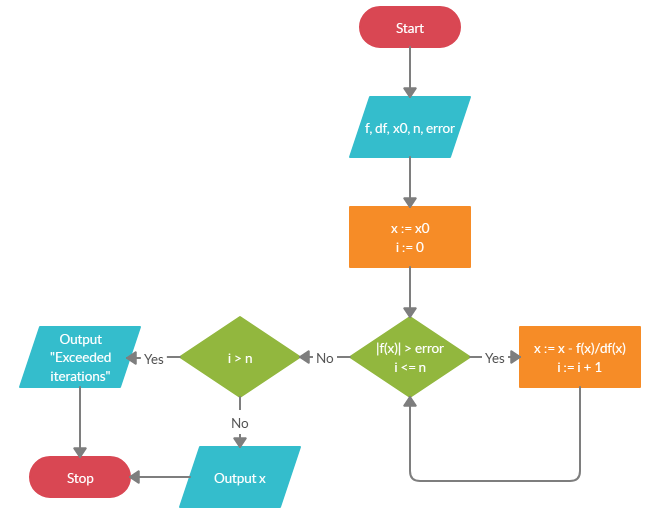
\includegraphics{newton.png}
\end{center}

Converting this flowchart to code gives the following:

\begin{verbatim}
==============================
def newton(f,df,x0,n,error):
	x = x0
	i = 0
        while abs(f(x)) > error and i <= n:
                x = x - f(x)/df(x)
                i += 1
        if i > n:
                return "Exceeded iterations"
        else:
                return x
==============================
\end{verbatim}

While Newton's Method may fail to converge, one reason to use it is that can converge to a solution faster than the Binomial Method.

\section{Problems}

All answers in this section have been rounded to the nearest thousandth and we have capped the number of iterations to 10.

\begin{question}
	Use Newton's Method to estimate the solution to $f(x)=0$ where $f(x)=x^3-7$ an error of at most 0.01. $\answer{1.914}$ 
\end{question}

\begin{question}
	Use the Newton's Method to give an approximation of $\sqrt{2}$ with an error of at most 0.01. $\answer{1.414}$
	\begin{hint}
		Find a simple function $f(x)$ such that $f(\sqrt{2})=0$ that is easy to work with.
	\end{hint}
	\begin{hint}
		Do not use $f(x)=x-\sqrt{2}$, as this would require an approximation of the number you wish to approximate.
	\end{hint}
\end{question}

\begin{question}
	Use the Bisection Method to give an approximation of the solution to the equation $x\ln{x}=4$ with an error of at most 0.01. $\answer{3.329}$
	\begin{hint}
		Remember to use \verb|import math| in order to use the logarithm.
	\end{hint}
\end{question}

\begin{question}
	Use the Bisection Method to give an approximation of all five of the solutions to $\ln{x}+\sin{x}=2$ on the interval $[5,20]$. Enter your solutions in increasing order. $\answer{6.424}$ $\answer{9.705}$ $\answer{12.061}$ $\answer{16.654}$ $\answer{17.779}$
	\begin{hint}
		Use a graphical tool (like Matplotlib) to get a sense for the locations of the solutions.
	\end{hint}
\end{question}

\section{Workspace}

\begin{sageCell}
# Use this cell to solve the above questions.
\end{sageCell}

\end{document}
